\documentclass[11pt,a4paper]{article}

\usepackage[margin=1in]{geometry}
\usepackage{titlesec}
\usepackage{enumitem}
\usepackage{hyperref}
\usepackage{parskip}
\usepackage{graphicx}
\usepackage{float}
\usepackage{booktabs}
\usepackage{amsmath}

\hypersetup{colorlinks=true, linkcolor=blue, urlcolor=blue}

\titleformat{\section}{\large\bfseries}{\thesection}{0.5em}{}
\titleformat{\subsection}{\normalsize\bfseries}{\thesubsection}{0.5em}{}
\setlist{leftmargin=1.4em, topsep=2pt, itemsep=2pt}

\title{\vspace{-1.5cm}\textbf{PKCERT AI \& Software Development Internship \\ Task 20: Feedforward Neural Network on Fashion-MNIST}}
\author{Abdullah Amir}
\date{AI and Software Development \\ 30 July 2026}

\begin{document}

\maketitle
\vspace{-0.8cm}

This report covers the theory and the results. The full code and outputs live in the
notebook \texttt{mnist\_feedforward.ipynb}. \textbf{PyTorch 2.13.0 (CPU build),
torchvision 0.28.0} are used throughout, random seed \textbf{42} fixed for the
train/validation split, model initialisation, and DataLoader shuffling. Tasks 18 and 19
built the network API fluency and training-loop mechanics used here; this task
assembles both into one complete, rigorously evaluated pipeline on
\textbf{Fashion-MNIST} (Xiao, Rasul \& Vollgraf, 2017), the stated MNIST alternative,
chosen because its confusion matrix is far more informative than plain MNIST's --
clothing categories with genuine visual overlap, rather than MNIST's mostly-solved
digit pairs.

% ----------------------------------------------------------------
\section*{Part A: Data Pipeline \& Preprocessing}

\textbf{Three-way split.} The official test set (10,000 images) is held out completely
until final evaluation. The official 60,000-image training set is further split
\textbf{50,000 (71.4\%) train / 10,000 (14.3\%) validation}, seed 42, so no
hyperparameter or epoch-count decision ever touches the test set.

\textbf{Normalization statistics, and the leakage they avoid -- demonstrated, not just
described.} Computed from the 50,000-image training split only: mean = 0.2857,
std = 0.3529. For comparison, computed from all 60,000 images (train+val together, the
leaky way): mean = 0.2860, std = 0.3530 -- a small but real difference (0.00029 in
mean). Using the leaked statistics would mean every training-time normalization already
encodes information about the exact 10,000 images later used for model selection; the
gap would only grow on a smaller dataset or a less i.i.d.\ split, so the principle
matters even when today's numeric impact is small.

\textbf{Pipeline shapes}, printed at every stage: raw PIL image $28\times28$ (mode L)
$\to$ after \texttt{ToTensor()}: $(1, 28, 28)$ $\to$ after flatten: $(784,)$ $\to$
batched tensor: $(128, 784)$, labels $(128,)$.

\begin{figure}[H]
    \centering
    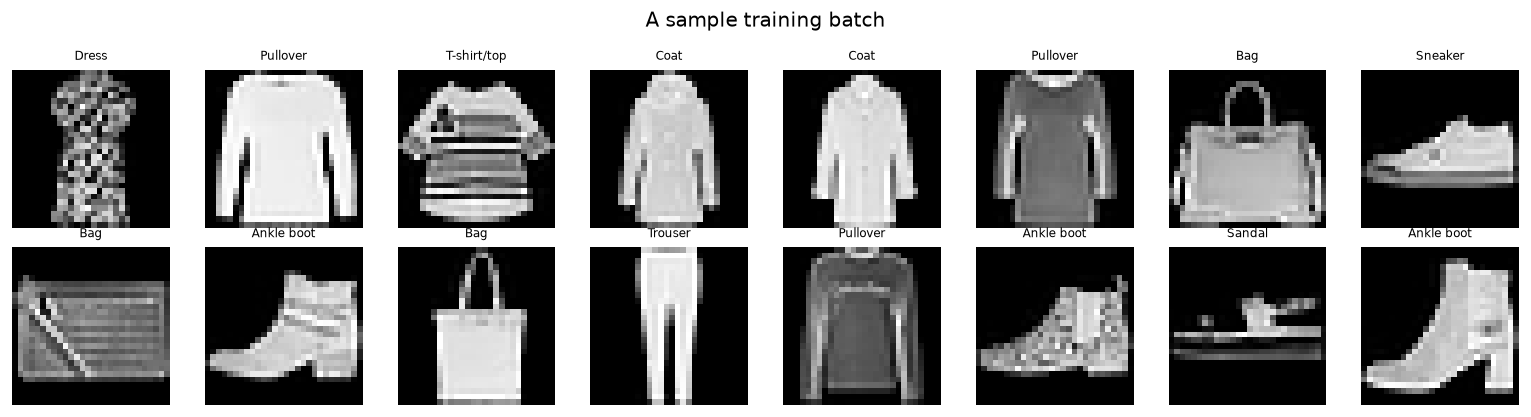
\includegraphics[width=0.95\textwidth]{figures/01_sample_batch.png}
    \caption{A sample training batch with true labels.}
\end{figure}

\textbf{Class distribution.} Reasonably but not perfectly balanced, as expected from a
non-stratified random split: the training split ranges from 4,926 to 5,055 images per
class (of 5,000 expected if perfectly even); validation and test are similarly close.

\begin{figure}[H]
    \centering
    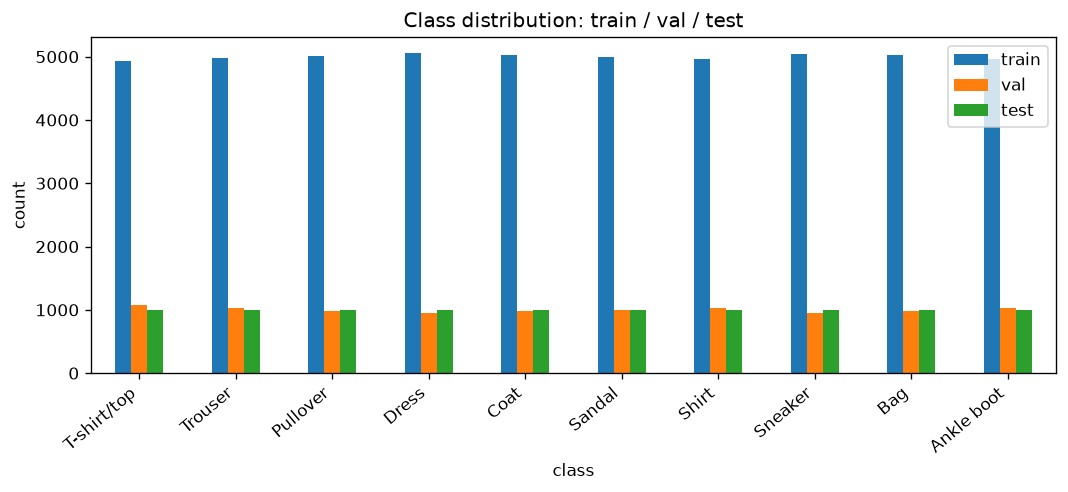
\includegraphics[width=0.85\textwidth]{figures/02_class_distribution.png}
    \caption{Class counts across the train / validation / test splits.}
\end{figure}

% ----------------------------------------------------------------
\section*{Part B: Model Architecture \& Design Justification}

\textbf{Architecture: $784 \to 256 \to 128 \to 10$} (3 fully-connected layers, 2
hidden). 256 (roughly a third of the 784-dimensional input) gives the first layer
enough width to form a broad bank of pixel-pattern detectors without the parameter
count exploding ($784\times256=200{,}704$ weights already dominates the model); 128
narrows that by half, compressing toward the 10-class output through an intermediate
representation. Two hidden layers, not more, was deliberate for a purely fully-connected
network (no weight sharing, unlike a CNN) on a 50,000-image training set: enough depth
to compose non-linear features, not so much that it overfits before the data can
constrain it.

\textbf{Activation: ReLU.} Sigmoid and tanh both saturate: their derivatives approach 0
as $|x|$ grows (sigmoid$'(x)$ peaks at only 0.25; tanh$'(x)$ peaks at 1.0 but still
decays fast). Backpropagation multiplies the upstream gradient by each layer's local
derivative, so stacking two such layers multiplies together two numbers usually well
below 1, shrinking the gradient reaching the first layer before training has even moved
it away from initialisation. ReLU's derivative is exactly 1 for any positive input, so
it passes gradient through unattenuated on its active side -- the deeper the stack, the
more this matters.

\textbf{Logits+CrossEntropyLoss vs softmax+NLLLoss, confirmed numerically equal.}

\begin{table}[H]
\centering
\begin{tabular}{lr}
\toprule
\textbf{Formulation} & \textbf{Loss on a sample batch} \\
\midrule
\texttt{CrossEntropyLoss(logits, y)} & 2.304028 \\
\texttt{NLLLoss(log\_softmax(logits), y)} & 2.304028 \\
\bottomrule
\end{tabular}
\caption{Identical to 6 decimal places -- CrossEntropyLoss literally computes log\_softmax then NLLLoss internally.}
\end{table}

Both formulations compute the mathematically identical quantity. The
logits+CrossEntropyLoss form is numerically preferred because it computes
$\log(\text{softmax}(z))$ directly via the log-sum-exp identity
($\log\text{softmax}(z)_i = z_i - \max(z) - \log\sum_j\exp(z_j-\max(z))$) in one fused,
stable operation, rather than computing softmax as an intermediate tensor (risking
underflow to exactly 0.0 for a confidently wrong logit) and taking its log separately.

\textbf{Parameter count, by hand and verified.}

\begin{table}[H]
\centering
\begin{tabular}{lrrr}
\toprule
\textbf{Layer} & \textbf{Weights} & \textbf{Biases} & \textbf{Total} \\
\midrule
784 $\to$ 256 & 200,704 & 256 & 200,960 \\
256 $\to$ 128 & 32,768 & 128 & 32,896 \\
128 $\to$ 10  & 1,280 & 10 & 1,290 \\
\midrule
\textbf{Hand-calculated total} & & & \textbf{235,146} \\
\texttt{sum(p.numel() for p in model.parameters())} & & & \textbf{235,146} \\
\bottomrule
\end{tabular}
\caption{Exact match.}
\end{table}

% ----------------------------------------------------------------
\section*{Part C: Training, Evaluation \& Experiments}

\textbf{Optimizer: Adam(lr=0.001), batch size 128, 20 epochs.} Task 19's own controlled
comparison found tuned SGD+momentum beating Adam on the small, 4-feature Palmer
Penguins network -- attributed there to Adam's adaptive scaling having no
uneven-gradient pathology to correct on such a small, well-conditioned problem. This
network is a different regime: 784 input dimensions of very unevenly informative pixels
(edge pixels are almost always 0, centre pixels carry most of the signal), closer to
the sparse/uneven-gradient case Task 19's worked example showed Adam handling better
than plain SGD. Batch size and epoch count were chosen as a standard, computationally
light starting point; the loss curves below confirm this was enough epochs to see
validation loss plateau.

\begin{figure}[H]
    \centering
    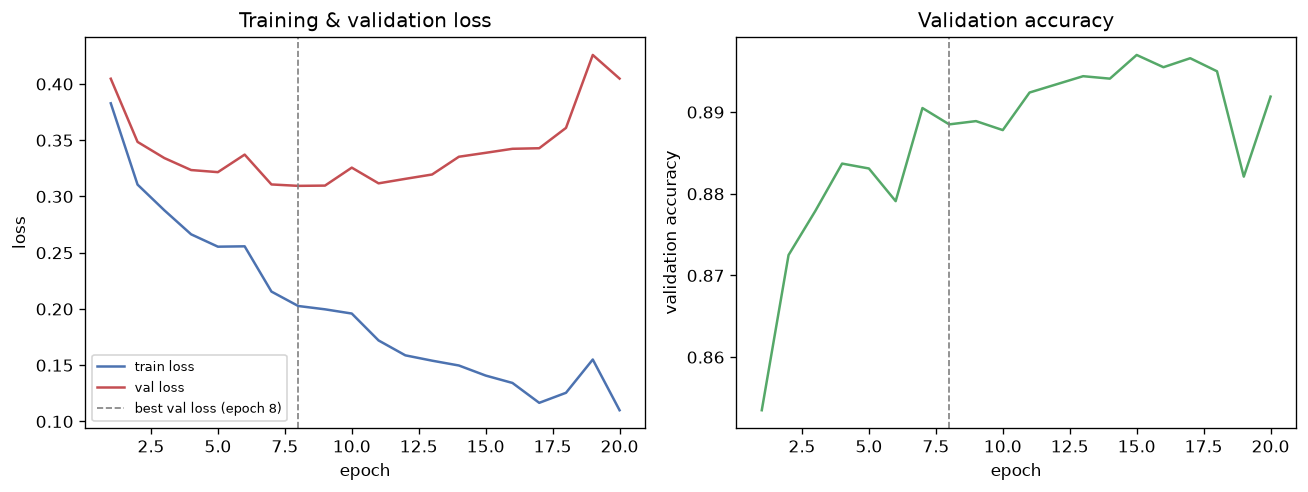
\includegraphics[width=0.95\textwidth]{figures/03_loss_accuracy_curves.png}
    \caption{Training/validation loss and validation accuracy across 20 epochs.}
\end{figure}

\textbf{Validation loss is lowest at epoch 8} (0.3094) and rises steadily afterward
(0.4048 at epoch 20) -- mild overfitting begins around epoch 8. Validation
\emph{accuracy}, however, keeps drifting upward with noise until around epoch 15, since
accuracy is a coarser, thresholded measurement than the continuous loss and can keep
improving slightly even as the model's confidence calibration (which loss penalises
directly) starts to degrade -- the two curves need not peak together.

\begin{table}[H]
\centering
\begin{tabular}{lr}
\toprule
\textbf{Metric (test set, 10,000 images)} & \textbf{Value} \\
\midrule
Accuracy & 0.8870 \\
Macro-Precision & 0.8880 \\
Macro-Recall & 0.8870 \\
Macro-F1 & 0.8873 \\
\bottomrule
\end{tabular}
\end{table}

\begin{figure}[H]
    \centering
    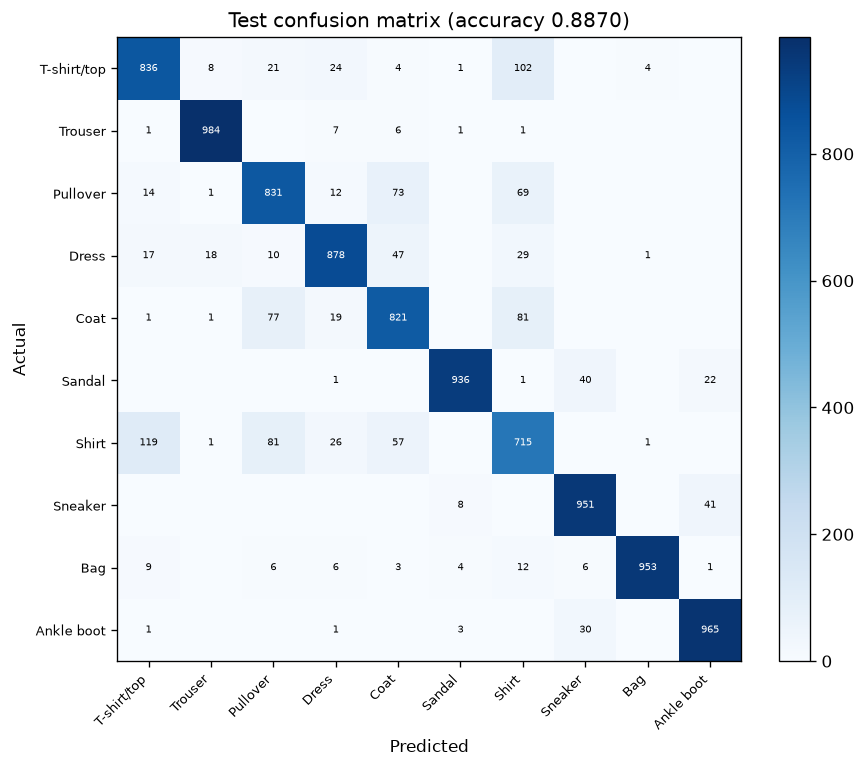
\includegraphics[width=0.72\textwidth]{figures/04_confusion_matrix.png}
    \caption{Test confusion matrix, all 10 classes.}
\end{figure}

\textbf{Shirt and T-shirt/top are the most confused pair}: 119 true-Shirt images
predicted T-shirt/top, 102 the reverse. Pullover/Coat/Shirt also cross-confuse
substantially (73, 81, 77, 81 off-diagonal counts among the three). All are upper-body
garments with overlapping silhouettes at $28\times28$ greyscale resolution, with no
colour or texture cue available to separate them -- exactly the kind of confusion a
purely fully-connected, spatially-blind network is expected to make.

\subsection*{Controlled ablation: network depth}

\begin{table}[H]
\centering
\begin{tabular}{lrr}
\toprule
\textbf{Configuration} & \textbf{Parameters} & \textbf{Test accuracy} \\
\midrule
0 hidden layers (linear) & 7,850 & 0.8417 \\
1 hidden layer (256) & 203,530 & 0.8797 \\
2 hidden layers (256, 128) & 235,146 & 0.8833 \\
\bottomrule
\end{tabular}
\caption{12 epochs each, identical seed, optimizer and batch size.}
\end{table}

\begin{figure}[H]
    \centering
    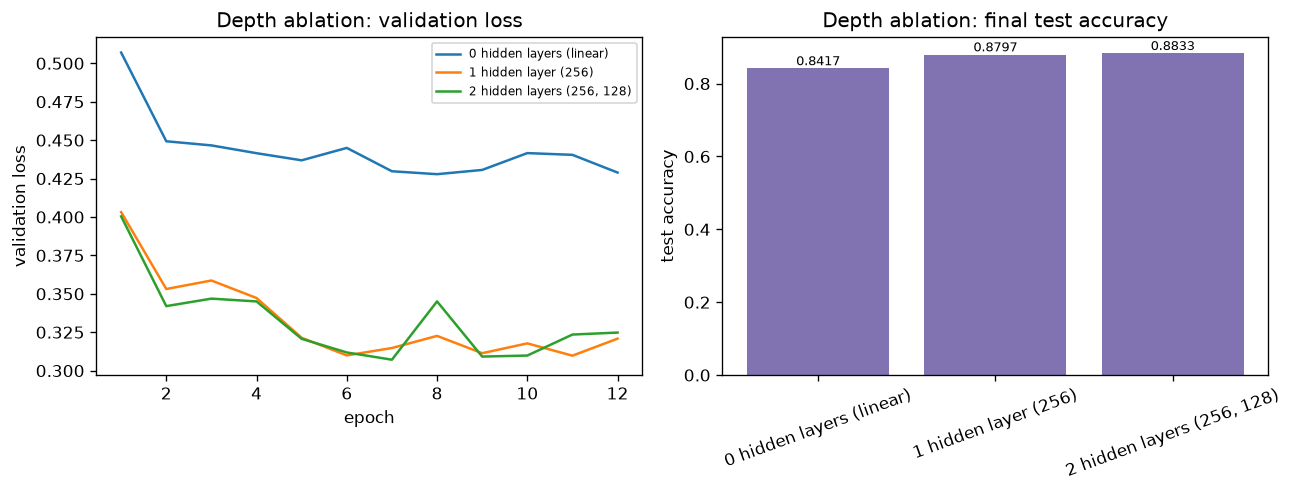
\includegraphics[width=0.95\textwidth]{figures/05_depth_ablation.png}
    \caption{Validation loss and final test accuracy across the depth ablation.}
\end{figure}

Adding the first hidden layer (0$\to$1) is worth \textbf{+3.80} points of test accuracy
for 195,680 more parameters; adding the second (1$\to$2) is worth only \textbf{+0.36}
points for 31,616 more parameters -- returned to in Part D.

\textbf{Model persistence, verified.} \texttt{torch.save(model.state\_dict(), ...)},
reloaded into a freshly-initialised model instance with \texttt{load\_state\_dict}:
predictions on a held-out batch were confirmed \textbf{exactly identical} to the
original model's, element for element.

% ----------------------------------------------------------------
\section*{Part D: Analysis \& Documentation}

\begin{table}[H]
\centering
\small
\begin{tabular}{lrrrrr}
\toprule
\textbf{Architecture} & \textbf{Params} & \textbf{Test Acc} & \textbf{Macro-P} & \textbf{Macro-R} & \textbf{Macro-F1} \\
\midrule
Linear (0 hidden) & 7,850 & 0.8417 & -- & -- & -- \\
1 hidden layer (256) & 203,530 & 0.8797 & -- & -- & -- \\
\textbf{2 hidden layers (256,128), main model} & \textbf{235,146} & \textbf{0.8870} & \textbf{0.8880} & \textbf{0.8870} & \textbf{0.8873} \\
\bottomrule
\end{tabular}
\caption{Precision/Recall/F1 computed for the main (20-epoch) model; the ablation
configurations (12 epochs) are scored on accuracy only, sufficient to isolate the effect
of depth. The main model's 2-hidden-layer test accuracy (0.8870) differs slightly from
the ablation's identical architecture (0.8833) purely because of the different epoch
budget (20 vs 12).}
\end{table}

\textbf{Counter-intuitive finding.} Going from one hidden layer to two barely moved test
accuracy (+0.36 points) \textbf{despite adding nearly as many parameters as the entire
first hidden layer contains} (31,616 new parameters vs 200,960 in the whole first
layer). The likely mechanism: a single 256-unit hidden layer already has more than
enough capacity to separate Fashion-MNIST's 10 classes given only 784 raw pixel inputs
-- the representational bottleneck was never depth, it was always the fact that raw
pixel intensities, even linearly recombined by one hidden layer's worth of ReLU units,
already capture most of the separable signal a fully-connected (no weight-sharing, no
spatial structure) network can extract. A second hidden layer adds parameters faster
than it adds separable signal once the first layer has already captured the easy wins --
the general shape of diminishing returns to depth in a plain MLP, and part of why
convolutional architectures, which use depth to build spatial hierarchies rather than
just stack more dense capacity, are the actual next step past this kind of network for
image data.

\textbf{A concrete implementation issue.} The normalization-leakage check in Part A was
not originally part of the plan -- it was added after the numbers needed independent
verification. An early version of this pipeline computed the normalization mean/std
from \texttt{raw\_train\_full.data} directly (all 60,000 images) before the train/val
split existed in the code, which is exactly the leakage Part A warns against. It was
caught by writing the leakage comparison \emph{deliberately}: computing the statistic
both ways (train-only vs full-60k) and checking that they should differ once the split
existed -- had a bug left the "train-only" computation silently identical to the full-set
one, that agreement itself would have been the signal that it was still touching data
outside the training split. The fix was a one-line reordering: compute
\texttt{train\_images} from \texttt{raw\_train\_full.data[train\_subset.indices]}
specifically, after the split is defined, not from the full tensor before it -- easy to
get backwards if the split and the normalization code are not read together as one
dependent unit.

\textbf{Reproducibility.} PyTorch 2.13.0 (CPU build), torchvision 0.28.0. Random seed 42
fixed for the train/val split, model initialisation, and DataLoader shuffling.
Optimizer: Adam, lr=$10^{-3}$. Batch size: 128. Epochs: 20 (main model), 12 (each
ablation configuration -- a shorter, deliberately lighter budget, past the point where
the depth ordering had stabilised).

\textbf{Conclusion.} Every claim in this report was checked against the pipeline's own
output rather than assumed: the leakage a full-dataset normalization would cause was
measured, not just described; both loss formulations were confirmed numerically
identical rather than asserted equivalent; the hand-calculated parameter count was
verified against PyTorch's own count; and the value of network depth was measured
directly rather than assumed monotonic -- which is exactly what surfaced the
diminishing-returns finding above. The result is an 88.70\% test-accuracy
fully-connected (no convolutions) classifier on Fashion-MNIST, with every design choice traceable to a
number from this pipeline's own run.

\vspace{0.4cm}
\noindent The notebook and README are on GitHub: {\small\scalebox{0.72}[1]{\url{https://github.com/AbdullahAmir06/ai-internship-abdullahamir}}}

\end{document}
